\chapter{基于邻边卷积网络的复合物筛选模型}
\label{chapter:EdgeConv}

本章首先介绍了生物数据对复合物预测的重要性,介绍了生物数据在蛋白质相互作用网络中的邻边嵌入。同时介绍了基于邻边嵌入的相关图卷积算法,并提出了基于邻边卷积网络的复合物筛选模型。最后针对该模型进行了相关的对比实验并分析了实验结果。

\section{引言}
\label{section:EdgeConv:Put}

已有方法已经充分表明,在PPI网络中进行蛋白质复合物预测不仅仅是一个图论中的聚簇发现问题,更是一个信息融合问题。无论是加权网络方法、核心附属结构预测方法,都致力于最大程度的利用生物学信息进行辅助预测。

而已有的算法通常将生物学信息,包括GO功能注释、拓扑域、亚细胞定位等转换为蛋白质之间的相似性数据,即映射为邻边数据。已有的基于加权图的复合物预测算法是将邻边特征映射到固定的权重计算公式中,相较于基于无权图的算法,其预测复合物的质量有较好的提升,说明邻边数据在复合物预测领域具有一定的重要性。

然而,硬编码的过程只能将丰富的生物数据进行简单的映射,无法做到对生物数据的高维抽象。
目前该研究领域尚未出现对邻边特征进行高维非线性抽象的算法。
基于以上前提,本文提出了利用生物特征基于邻边卷积网络的复合物局部子图分类模型。

\section{邻边卷积网络介绍}
\label{section:EdgeConv:intro}

邻边卷积网络\cite{wang_dynamic_2019}(EdgeBase Convolution)由点云学习领域提出,是一种基于邻边做特征转换以及特征聚合的方法。点云学习指的是使用计算机的方法学习与分析空间中独立数据点的集合,数据点的信息包括坐标、颜色、分类、强度值等等信息,数据点在空间中的集合状态即为点云。点云学习的任务是对点云数据做分割、物体识别等等。

在点云任务中,会与待更新结点i周围的K个最近邻居建立连边,基于连边做特征更新,然后所有的连边特征汇聚到一起作为结点的新特征。连边特征更新的过程中会考虑源点与汇点的信息流动,其具体的过程如图\ref{fig:edgeconv_main}所示。
\begin{figure}[htbp]
    \centering
    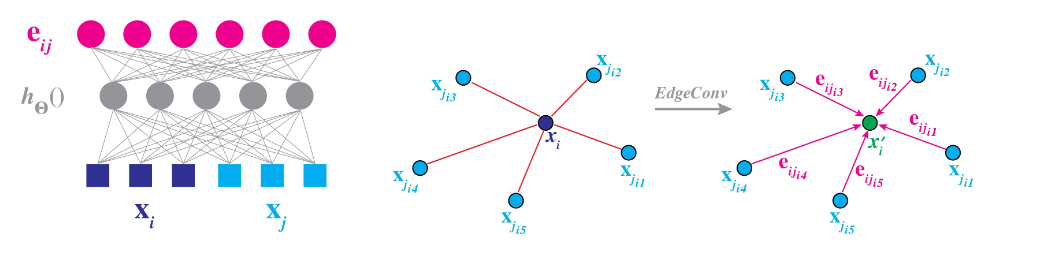
\includegraphics[width=14cm]{edgeconv_main}
    \caption{基于邻边的图卷积神经网络更新示意图\cite{wang_dynamic_2019}}
    \label{fig:edgeconv_main}
\end{figure}

对于结点i的更新,需要从结点i周围的5个邻居建立到结点i的邻边。对于其中某一条邻边$E_{j,i}$,其两个端点分别具有各自的特征,将特征拼接到一起,然后经过邻边卷积的多层感知器计算,即可得到邻边特征更新后的结果$e_{ij}$如图中左侧所示。
更新结点i周围所有的邻边特征,然后计算其和值,就形成了结点i更新之后的特征,如图\ref{fig:edgeconv_main}中右侧所示。

\section{基于邻边卷积网络的复合物筛选模型}
\label{section:EdgeConv:detail}
本节分别介绍基于邻边卷积单层更新的具体实现,以及基于该单层更新方法构建的蛋白质复合物评价模型,最后介绍复合物筛选模型的总体实现流程。

\subsection{基于邻边卷积单层更新}
\label{subsection:EdgeConv:single}

在通常的图卷积过程中,结点A的特征为周围所有结点的特征和自生特征决定,可以采取平均值的计算方法,如公式\ref{equ:NormalGCNNodeFlow}所示。
\begin{equation}
    \label{equ:NormalGCNNodeFlow}
    f_a=\delta (\frac{\sum_{i = 1}^{n}f_i+f_a}{n+1})
\end{equation}
其中$f_a$代表A结点的特征,$f_i$代表A结点所有邻居的特征,$\delta$为信息汇聚之后的特征更新函数。

在基于邻边卷积的复合物预测方法中,结点特征更新由其邻边共同决定。其具体计算过程如公式\ref{equ:EdgetoNodeFeat}所示。
\begin{equation}
    \label{equ:EdgetoNodeFeat}
    f_a=\delta (\frac{\sum_{i = 1}^{n}f_{ia}}{n})
\end{equation}
其中$f_{ia}$表示所有连接到A的邻边特征。其具体的汇聚过程如图\ref{fig:edge-feat-flow}所示,A结点汇聚周围所有邻边特征,包括$F_{BA}$、$F_{CA}$、$F_{DA}$以及$F_{EA}$。

\begin{figure}[htbp]
    \centering
    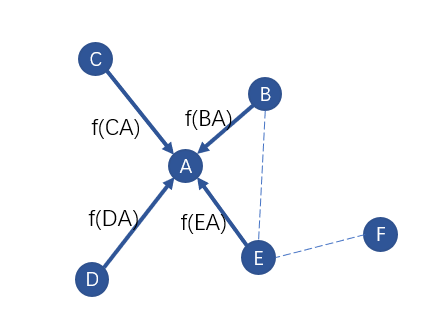
\includegraphics[width=7cm]{edge-feat-flow}
    \caption{边特征初始化结点特征示意图}
    \label{fig:edge-feat-flow}
\end{figure}

蛋白质生物数据是基于邻边的数据,因此在对复合物子图做图卷积的时候,基于生物特征的模型采用了基于edge的GCN模型\cite{wang_dynamic_2019},其具体的邻边更新方式如式\ref{equ:EdgeConv}所示。
\begin{equation}
    \label{equ:EdgeConv}
    %\max_{j \in \mathcal{N}(i)} 
    e_{ij}^{(l)} = \mathrm{LeakyReLU}(
    \Theta \cdot (h_j^{(l)} - h_i^{(l)}) + \Phi \cdot h_i^{(l)})
\end{equation}
其中$e_{ij}^{(l)}$表示第$l$层邻边更新之后的特征数据,$h_j^{(l)} - h_i^{(l)}$表示从邻居结点到$i$结点的数据流,$h_i^{(l)}$为结点保留信息,$\Theta$和$\Phi$分别对应更新函数。$LeakyRelu$为邻边特征激活函数。

结点更新的方式如式\ref{equ:EdgeConv-node}所示,
\begin{equation}
    \label{equ:EdgeConv-node}
    %\max_{j \in \mathcal{N}(i)} 
    h_j^{(l+1)} = \max(h_j^{(l)},\frac{\sum_{i \in N(j)}{e_{ij}^{(l)}}}{\left\lVert N(j)\right\rVert } )
\end{equation}
式中$h_j^{(l+1)}$为第第$l+1$层结点j更新之后的特征数据,$N(j)$表示结点的所有邻居,$\left\lVert N(j)\right\rVert $表示邻边数量,$e_{ij}^{(l)}$表示某一条邻边更新之后的特征。

每一轮基于edgeConv的卷积过程可以图\ref{fig:edgeconv_edgeconv}所示,结合公式和图片,可以得出基于edgeConv的卷积过程首先是由结点更新邻边特征,如图中上半部分所示,在子图中每一条邻边特征会获取其两个端点(源点和汇点)的特征,第一部分更新为源点至汇点的特征相减并做特征转换,代表邻边的数据流,第二部分为源点特征做特征转换,这两部分特征结合到一起经过激活形成邻边更新的特征。然后是用更新之后的邻边特征聚合物新的结点特征,如图中下半部分所示,结点会汇聚其所有邻边的特征并取平均值,同时依据最大值池化结点会保留一部分自身特征。

\begin{figure}[htbp]
    \centering
    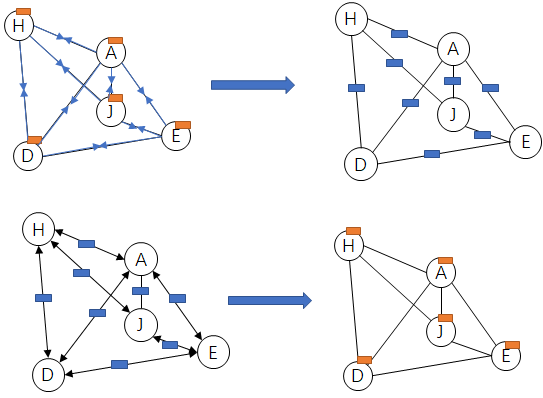
\includegraphics[width=10cm]{edgeconv_edgeconv}
    \caption{总体EdgeConv图卷积过程示意图}
    \label{fig:edgeconv_edgeconv}
\end{figure}

\subsection{特征子图评价模型}

本文处理了大量的生物学数据,包括蛋白质功能注释数据、结构域相互作用数据、亚细胞定位数据等,应用相关的生物领域的处理方法将生物学数据转换为可应用的特征数据,最终得到了11维度的特征数据。所有的特征都描述蛋白质相互作用,因此在图结构中,这些特征编码为图结构邻边的特征。
基于邻边卷积特征的复合物筛选模型总体流程如图\ref{fig:edgeconv_flow}所示。

第一阶段如标号1所示,需要将初始的邻边特征以汇聚方法初始化结点特征,如图中上半部分所示。该汇聚方法为初始结点特征由其周围所有邻边特征的平均值替代。其具体的计算过程如公式\ref{equ:EdgetoNodeFeat}所示,其中激活函数为直接映射。其过程可被视为聚合阶段的基于边卷积神经网络过程,如图中\ref{fig:edgeconv_edgeconv}下半部分所示。

第二阶段如标号2所示,需要基于邻边卷积将特征与拓扑结构融合,基于pool方法得到子图结构的特征表示,并基于子图特征做分类预测以及评分预测。其具体过程如图中下半部分所示。

模型使用了两层的基于邻边卷积的图神经网络,图卷积过程中隐层维度设置为64维。
两层图卷积之后,采用了对结点特征分别做最大值池化和平均值池化的方法,拼接到一起得到128维的子图特征。后续分别为两层感知器和softmax层得到图的分类预测,两层感知器和sigmoid层得到图的评分预测。


\begin{figure}[htbp]
    \centering
    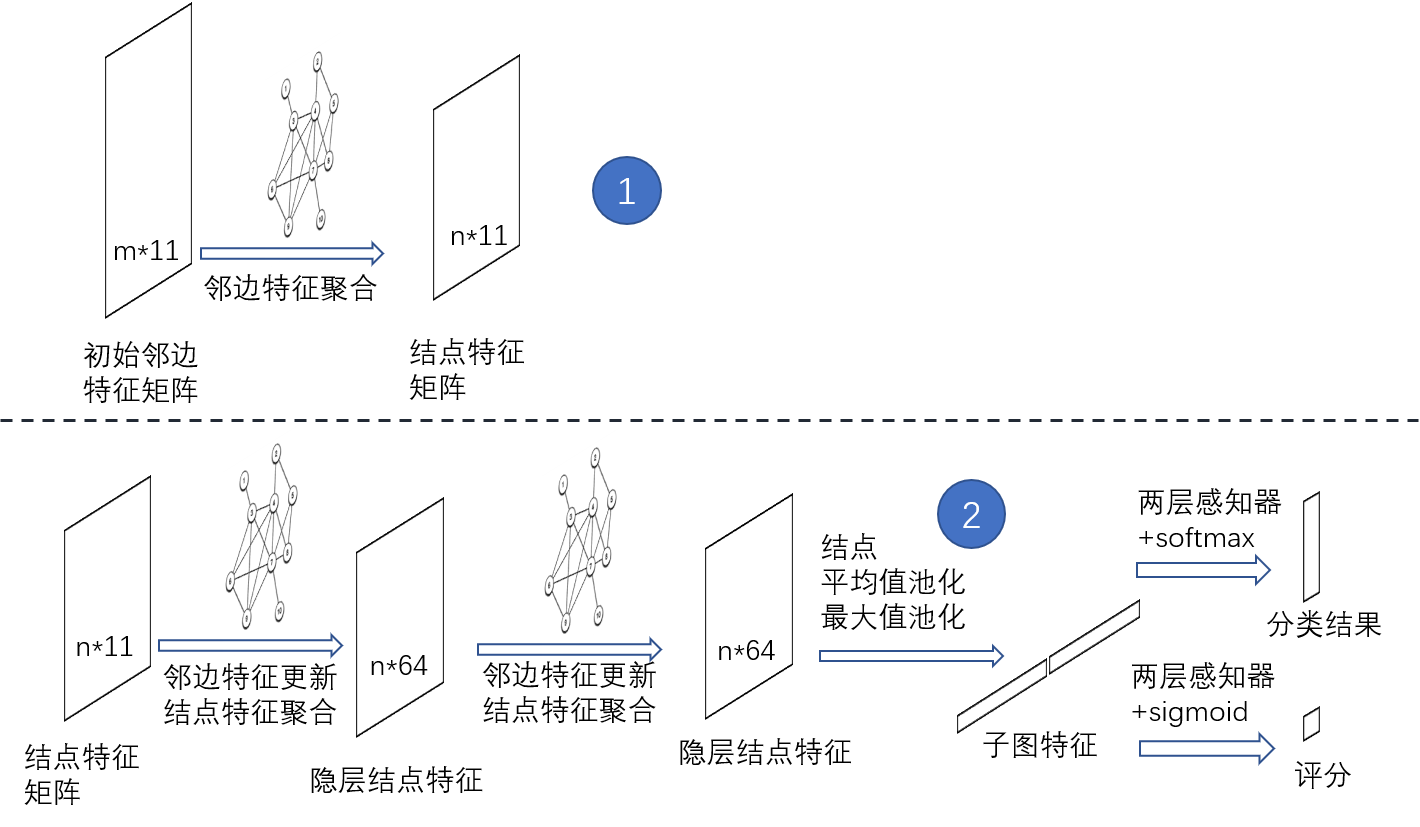
\includegraphics[width=15cm]{edgeconv_flow}
    \caption{基于邻边卷积特征的复合物筛选模型总体流程}
    \label{fig:edgeconv_flow}
\end{figure}

\subsection{筛选模型算法}
本节介绍基于邻边卷积的复合物筛选模型的具体算法,包括数据处理,模型训练,样本筛选与结果比对。
具体如算法\ref{alg:edgegcn-screen}所示。

\begin{algorithm}[h]
    \caption{Protein complex screening model based on edge convolution} % 名称
    \label{alg:edgegcn-screen}
    \begin{algorithmic}[1]
        \Require
        $Com_t$: train protein complexes;
        $Com_b$: protein complexes before screen;
        $Com_g$: golden bench protein complexes;
        $G$: protein-protein interaction network
        \Ensure
        $F1_a,F1_b/SPA_a,SPA_b$: predicted protein complexes F1/SPA metrix after and before screen;
        \State $n$:PIN node number;$m$:PIN edge number;$Com_a=None$;
        \State $F_{GO}\in \mathbb{R}^{m\times 2},F_{DDI}\in \mathbb{R}^{m\times 7},F_{Subcell}\in \mathbb{R}^{m\times 2}$;
        \State $F_{E} \in \mathbb{R}^{m\times 11}=Concat(F_{GO},F_{DDI},F_{Subcell})$;
        \State $Subs_t=Ext(G,F_{E},Com_t)$: feated subgraph extract algorithm;
        \For{i=0;i<epoch;i++}
        \For{$BSub_t \in Sub_t$} $loss=0$;
        \For{$Sub_t \in BSub_t$}
        \State $F_{N}^0 =Linear_m(Mean(Neighbor(F_{E}))), \in \mathbb{R}^{m_{sub}\times 11}$;
        \State $F_{N}^1=EdgeConv^0(G,F_{N}^0), \in \mathbb{R}^{m_{sub}\times 64}$
        \State $F_{N}^2=EdgeConv^1(G,F_{N}^1), \in \mathbb{R}^{m_{sub}\times 64}$
        \State $F_t=Concat(MeanP(F_{N}^2),Maxp(F_{N}^2)), \in \mathbb{R}^{m_{sub}\times 128}$;
        \State $PredC_t=MLP_C(F_t),\in \mathbb{R}^{1\times 4}$;$PredS_t=MLP_S(F_t),\in \mathbb{R}^{1}$;
        \State $loss+=\{CEL(PredC_t,LabelC_t)+\alpha \cdot BCEL(PredS_t,LabelS_t)\}$
        \EndFor; optimization $Adam(loss)$;
        \EndFor
        \EndFor
        \State $Subs_b=Ext(G,F_{E},Com_b)$: feated subgraph extract algorithm, see in \ref{section:featSubNetworkConstruct:allSample};
        \For{$Sub_b \in Subs_b$} $PredC_b=MLP_C(F_b)$;$PredS_b=MLP_S(F_b)$;
        \State $Com_a+=Complex(Sub_b)~if~PredC_b=positive|PredS_b>=0.25$;
        \EndFor
        \State $F1_a=F1(Com_a,Com_g),F1_b=F1(Com_b,Com_g)$;
        \State $SPA_a=SPA(Com_a,Com_g),SPA_b=SPA(Com_b,Com_g)$;
    \end{algorithmic}
\end{algorithm}
模型算法中输入数据包括本文\ref{section:featSubNetworkConstruct:allSample}节构造的训练数据集$Com_t$、待筛选数据集$Com_b$以及蛋白质相互作用网络图结构数据,其中训练数据集由蛋白质复合物的正样本数据集,中间样本数据集和负样本数据集构成,训练数据集中每一个蛋白质符合物样本均具有分类标注与评分标注。

模型的输出数据为待筛选数据集筛选之前的所有样本$Com_b$与筛选之后剩余样本$Com_a$的评价指标,评价指标需要参照真实复合物样本集$Com_g$计算,计算的指标包括F1值和综合评价指标SPA。最终的输出为筛选后F1评价指标$F1_a$、筛选前F1评价指标、筛选后SPA评价指标$SPA_a$、筛选前SPA评价指标$SPA_b$,如算法中输出部分所示。

算法中第2行代表采用多种蛋白质相似性特征计算方法嵌入的邻边特征,其中包括基于GO相似性得到的2维特征$F_{GO}\in \mathbb{R}^{m\times 2}$,基于蛋白质拓扑域相似性得到的7维特征$F_{DDI}\in \mathbb{R}^{m\times 7}$以及基于蛋白质亚细胞定位得到的2维特征$F_{Subcell}\in \mathbb{R}^{m\times 2}$,这些特征具体的计算方法如\ref{subsection:featPPINetwork:edgeFeatConstruct}所示。通过$Concat$的方法将三种蛋白质相似性特征拼接到一起,得到11维的特征矩阵$\mathbb{R}^{m\times 11}$,如第3行所示,其中m表示的是蛋白质相互作用网络中的所有连边数量。算法中第4行和第17行表示结合互作网络,特征数据和蛋白质复合物中的蛋白质集合提取取蛋白质复合物特征子图的方法,其中$Subs_t$表示训练数据集提取的所有特征子图,$Subs_b$为待筛选数据集提取的所有特征子图,其具体实现如\ref{section:featSubNetworkConstruct:allSample}所示。

第5行至第16行表示基于邻边卷积的蛋白质评价模型的训练过程,模型采用分批次的训练方法,同一个批次的若干子图训练损失加和作为整个批次的损失,并进行批次更新参数,如第13行和14行所示。算法中第8行为基于邻边特征转换为结点特征的算法,其具体过程为遍历子图中的每一个结点,将结点特征初始化为其所有邻边的特征和,具体计算方法如\ref{equ:EdgetoNodeFeat}所示,然后基于一层神经网络进行特征转换得到结点初始化特征,该神经网络的参数为$\mathbb{R}^{11\times 11}$。
第9行和第10行表示两层基于邻边卷积过程。对于单层邻边卷积神经网络,其更新过程为邻边特征更新与结点特征汇集,邻边特征更新为两个方面的和,分别为数据流更新和源点特征更新,结点特征汇集包括为两个方面的最大值,分别为自身特征和邻边特征平均值,其更新的具体过程如\ref{subsection:EdgeConv:single}所示。由于数据维度的不同,$EdgeConv_0$更新网络的参数规模为$\mathbb{R}^{11\times 64}$,$EdgeConv_1$更新网络的参数规模为$\mathbb{R}^{64\times 64}$。

第11行表示图读出过程,由于在该模型中邻边特征初始化为了结点特征,同时结点特征经过两层邻边卷积神经网络已经和子图拓扑结构进行了融合,此时结点特征具有较强的表达能力,隐层隐层图读出采用所有结点隐层特征的最大池化$Maxp$和平均池化$Meanp$拼接$Concat$作为子图的特征。

第12行表示以基于子图特征的分类预测与评分预测。
第18行至第22行表示基于以训练模型筛选蛋白质复合物样本以及评价阶段。其具体细节如算法\ref{alg:nodegcn-screen}描述所述。


\section{实验设计及结果分析}
\label{section:EdgeConv:experience}

为了验证生物特征的添加对算法模型的提升,本文对比了在不添加生物数据,而使用相同的GCN结构的情况下,复合物分类模型对样本质量的提升程度。

\subparagraph*{实验方案(一)} 稀疏网络中基于邻边卷积筛选模型实验

在本文介绍的四个$PPI$网络中,DIP网络的密度最低,为0.0014,其平均度数最低6.98,具有一定的稀疏性。且DIP网络的结点数量较多,为4928个,仅次于Biogrid网络,数据完整性较高。因此方案(一)选择DIP网络作为稀疏网络进行相关实验。

\begin{figure}[htbp]
    \centering
    \subcaptionbox{F1值对比}{\label{fig:dip_f1_edge}
        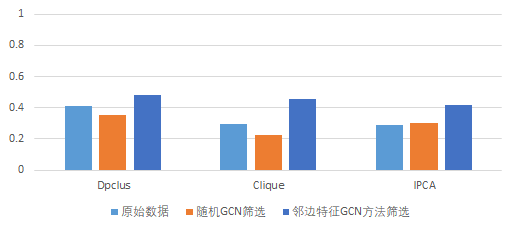
\includegraphics[width=10cm]{dip_f1_edge}}
    \vskip0.2cm
    \subcaptionbox{SPA值对比}{\label{fig:dip_spa_edge}
        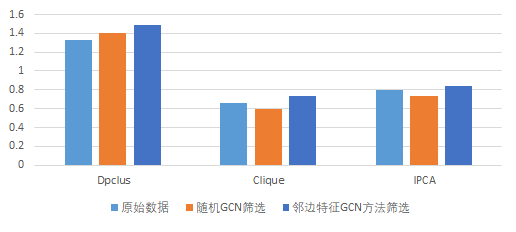
\includegraphics[width=10cm]{dip_spa_edge}}
    \caption{DIP网络不同模型处理后结果对比}
    \label{fig:dip_edge}
\end{figure}

\begin{table}[h]
    \centering
    \caption{DIP网络不同模型处理后结果对比数据}
    \begin{tabular}{C{2cm}C{2cm}C{2cm}C{2cm}}
        \toprule
        \textbf{F1值} & \textbf{原始数据} & \textbf{随机GCN筛选} &\textbf{邻边特征GCN筛选} \\
        \midrule
        Dpclus算法    & 0.414             & 0.352                & 0.484                                 \\
        Clique算法    & 0.296             & 0.222                & 0.453                              \\
        IPCA算法      & 0.291             & 0.300                & 0.420                               \\
        \bottomrule
    \end{tabular}
    \begin{tabular}{C{2cm}C{2cm}C{2cm}C{2cm}}
        \toprule
        \textbf{SPA值} & \textbf{原始数据} & \textbf{随机GCN筛选} & \textbf{邻边特征GCN筛选} \\
        \midrule
        Dpclus算法     & 1.333             & 1.340                & 1.490                                    \\
        Clique算法     & 0.658             & 0.596                & 0.731                                  \\
        IPCA算法       & 0.794             & 0.729                & 0.838                               \\
        \bottomrule
    \end{tabular}
    \label{tab:result/DIP/edge}
\end{table}

依据\ref{section:NodeConv:experience}部分中实验方案(一)中提到的方法,针对DIP网络构造了具有四类分类的训练特征子图数据集,基于三种方法生成了待筛选复合物数据集。实验中在训练特征子图数据集基础上训练了基于邻边卷积网络的评价模型。模型训练完成之后,分别对三个待筛选特征子图样本数据集中的样本进行了测试并将其中符合要求的复合物保留下来,作为筛选后样本数据集。接下来分别对比了筛选前后样本数据集F1值和综合评价指标。

按照以上的实验方法本章对比了基于随机邻边特征的邻边卷积模型,随机邻边特征模型的对比可以确定嵌入的邻边相似性特征的有效性,本章总体的实验结果如下所示。

图\ref{fig:dip_edge}为在DIP网络中,随机特征模型和基于生物特征的模型筛选之后结果的对比,包含了F1值对比图和SPA值对比图。表\ref{tab:result/DIP/edge}为实验结果具体数据。


\subparagraph*{实验方案(二)} 稠密网络中基于邻边卷积筛选模型实验

在本文介绍的四个$PPI$网络中,Biogrid网络的密度最高,为0.0038,其平均度数最低21.40,远高于其他$PPI$网络,相较于其他网络Biogrid网络稠密性较高。且Biogrid网络的具有最高的结点数量,数据为5573。因此方案(二)选择Biogrid网络作为稠密网络进行相关实验。


\begin{figure}[htbp]
    \centering
    \subcaptionbox{F1值对比}{\label{fig:biogrid_f1_edge}
        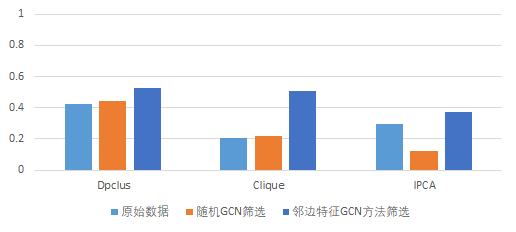
\includegraphics[width=10cm]{biogrid_f1_edge}}
    \vskip0.2cm
    \subcaptionbox{SPA值对比}{\label{fig:biogrid_spa_edge}
        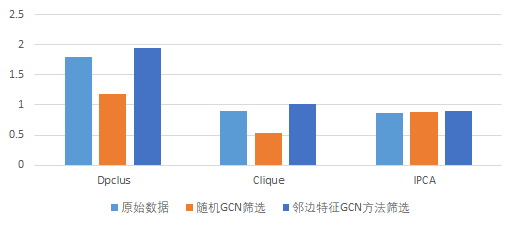
\includegraphics[width=10cm]{biogrid_spa_edge}}
    \caption{Biogrid网络不同模型处理后结果对比}
    \label{fig:biogrid_edge}
\end{figure}

\begin{table}[h]
    \centering
    \caption{Biogrid网络不同模型处理后结果对比数据}
    \begin{tabular}{C{2cm}C{2cm}C{2cm}C{2cm}}
        \toprule
        \textbf{F1值} & \textbf{原始数据} & \textbf{随机GCN筛选} &\textbf{邻边特征GCN筛选} \\
        \midrule
        Dpclus算法    & 0.425             & 0.445                & 0.529                                 \\
        Clique算法    & 0.203             & 0.216                & 0.510                              \\
        IPCA算法      & 0.294             & 0.122                & 0.373                               \\
        \bottomrule
    \end{tabular}
    \begin{tabular}{C{2cm}C{2cm}C{2cm}C{2cm}}
        \toprule
        \textbf{SPA值} & \textbf{原始数据} & \textbf{随机GCN筛选} & \textbf{邻边特征GCN筛选} \\
        \midrule
        Dpclus算法     & 1.796             & 1.119                & 1.950                                    \\
        Clique算法     & 0.901             & 0.532                & 1.011                                  \\
        IPCA算法       & 0.859             & 0.886                & 0.891                               \\
        \bottomrule
    \end{tabular}
    \label{tab:result/Biogrid/edge}
\end{table}


依据\ref{section:NodeConv:experience}部分中实验方案(二)中提到的方法,针对Bigrid网络构造了具有四类分类的训练特征子图数据集,基于三种方法生成了待筛选复合物数据集。实验中训练了基于邻边卷积网络的评价模型,并分别对三个待筛选特征子图样本数据集中的样本进行了测试,获取了筛选后样本数据集,最后对比了筛选前后样本数据集F1值和综合评价指标。

按照以上的实验方法本章对比了基于随机邻边特征的邻边卷积模型,随机邻边特征模型的对比可以确定嵌入的邻边相似性特征的有效性,本章总体的实验结果如下所示。
图\ref{fig:biogrid_edge}为在Biogrid网络中,随机特征模型和基于生物特征的模型筛选之后结果的对比,包含了F1值对比图和SPA值对比图。表\ref{tab:result/Biogrid/edge}为实验结果具体数据。

\subparagraph*{实验结论} ~

从实验方案(一)从图中可以看出,添加了生物特征后,在DIP网络中复合物的生成质量得到了相应的提升,同样的由于CLique算法的特性,该算法的前后对比提升幅度最为明显。
和实验方案(二)从图\ref{fig:biogrid_edge}中可以看出添加了生物特征后,Biogrid网络相应样本的F1值均有较为明显的提升,而Clique算法的样本提升最为明显。综合评价指标SPA值也具有一定的提升。

基于相似性数据邻边嵌入的复合物筛选模型,对比无相似性嵌入模型取得较高的F1值和SPA值提升,稠密网络具有更多的邻边信息,在稠密网络中其提升幅度更为明显,最高的F1值提升在Biogrid的Clique算法中,从0.203提升至0.510。


\section{本章小结}
\label{section:EdgeConv:summary}

本章基于蛋白质相似性特征出发,提出了使用基于邻边卷积的复合物特征子图评价模型以及相应的筛选算法。通过多种蛋白质相似性计算方法为蛋白质复合物子图嵌入11维度的邻边特征,提出了邻边特征初始化结点特征的方法以及蛋白质复合物中基于邻边卷积的信息流更新过程。最后本章对比了基础的无特征邻边卷积模型,实验结果表明了生物相似性特征和筛选模型的有效性以及邻边卷积对特征数据具有融合能力。